\documentclass[12pt,a4paper]{article}
\usepackage[utf8]{inputenc}
\usepackage[spanish]{babel}
\usepackage{amsmath}
\usepackage{amsfonts}
\usepackage{amssymb}
\usepackage{makeidx}
\usepackage{hyperref}
\usepackage{graphicx}
\usepackage{fancyhdr}
\usepackage{wrapfig}
\usepackage{float}
\usepackage{placeins}
\usepackage{afterpage}
\usepackage[left=2cm,right=2cm,top=2cm,bottom=2cm]{geometry}
\graphicspath{ {./images/} }

\title{Gymodo}

\pagestyle{fancy}
\fancyhf{}
\rhead{Gymodo}
\lhead{M13 Proyecto Desarrollo de aplicaciones multiplataforma}
\fancyfoot[C,CO]{\leftmark}
\fancyfoot[L,RO]{\thepage}

\renewcommand{\headrulewidth}{2pt}
\renewcommand{\footrulewidth}{1pt}

\begin{document}

\begin{titlepage}
    \begin{center}
        \vspace*{1cm}
            
        \Huge
        \textbf{Gymodo}
            
        \vspace{0.5cm}
        \LARGE
        La mejor App para tu gym
        
        
\includegraphics[width=\textwidth]{gymodo_logo}
        
        \vfill
        

        Edgar Luque, Shah Sawar, Ronald Intriago\\
            
        \vspace{0.8cm}
           
            
        \Large
        Desarrollo de Aplicaciones Multiplataforma\\
        Escola del Treball\\
        Barcelona\\
        \today
            
    \end{center}
\end{titlepage}

\newpage

\begin{abstract}
Gyomodo es una aplicación que tiene como objetivo resolver los problemas que puedan tener los gymnasios en estos tiempos modernos, pero sobretodo, problemas originados a partir de la pandemia del Covid-19.

Este documento explica el desarrollo de esta aplicación, su funcionalidad y la organización del equipo.
\end{abstract}

\newpage

\tableofcontents

\newpage

\section{Presentación del proyecto}
Este proyecto se basa en el desarrollo de una aplicación para Android, esta aplicación tiene como objetivo principal cubrir las necesidades digitales que puede tener un gimnasio como:

\begin{itemize}
\item Crear rutinas y ejercicios.
\item Reservar una hora para ir al gimnasio.
\item Crear tus propias dietas y escanear el código de barras de los productos para ver su nutrientes.
\item Ver noticias relacionadas con el mundo del ejercicio.
\end{itemize}

\newpage

\section{Estructura y Organización}
TODO EXPLICAR ORGANIZACION AQUI

\newpage

\section{Tecnología usada}

\subsection{Organización}

\begin{wrapfigure}{R}{0.25\textwidth}
  \centering
    
\includegraphics[width=\linewidth]{asana}
  	\bigskip\par
  	 
\includegraphics[width=\linewidth]{toggl}
  	\bigskip\par
   
\includegraphics[width=\linewidth]{git}
   \bigskip\par
    
\includegraphics[width=\linewidth]{androidstudio}
   \bigskip\par
\end{wrapfigure}

\subsubsection{Asana}

Para organizar las tareas que tenemos que hacer hemos empleado Asana, una aplicación web que permite organizar el trabajo.


Con Asana podemos crear tareas, sub-tareas y asignarlas a cada uno, también permite poner un tiempo limite. 

\subsubsection{Toggl}
Para saber el tiempo empleado en cada tarea usamos la herramienta toggl tracker.

\subsection{Desarrollo}

\subsubsection{Control de Versiones}

El sistema de control de versiones que hemos usado es git, gracias a esta herramienta podemos mantener el proyecto de forma eficiente, este es nuestra forma de trabajar:

\begin{enumerate}
\item Actualizar la branca rama principal
\item Crear una rama donde guardaras tu nuevo trabajo.
\item Hacer el trabajo y subirlo.
\item Otro miembro revisa el código y si esta bien se hace un merge a la rama principal.
\item Repetir el paso 1.
\end{enumerate}

\subsubsection{Android Studio}
Para desarrollar la aplicación hemos usado el IDE Android Studio.
Este IDE es el estándar de la industria para crear aplicaciones de Android, esta desarrollada por Google y Jetbrains.


\newpage

\section{Análisis funcional}

\newpage

\subsection{Diagrama UML}

\begin{figure}[h]
 	\centering
	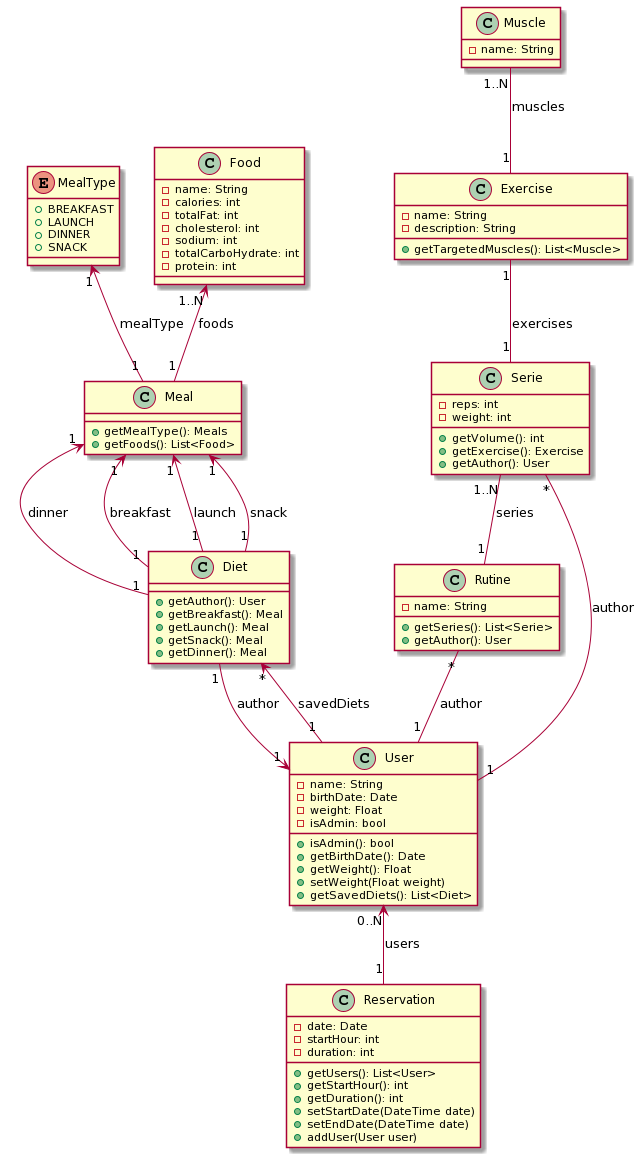
\includegraphics[width=0.6\textwidth]{uml}
	\caption{Diagrama UML}
\end{figure}

\newpage

\subsection{Diagrama Casos de Uso}

\begin{figure}[h]
 	\centering
	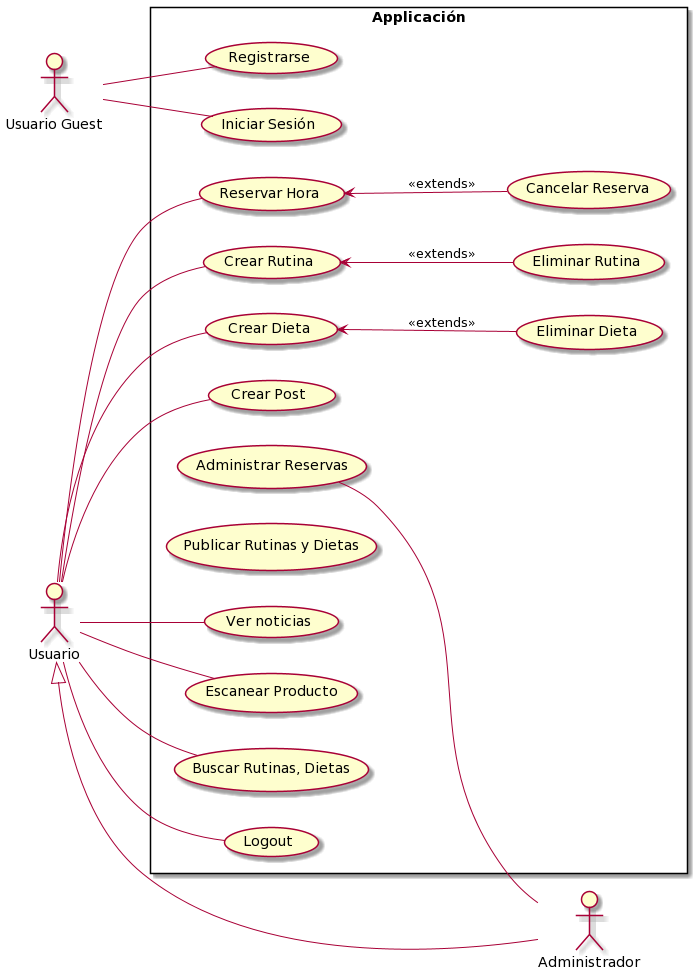
\includegraphics[width=0.6\textwidth]{casos_uso}
	\caption{Diagrama de Casos de Uso}
\end{figure}

TODO: Explicar casos de uso paso a paso. e.g: 1. seleccionar boton x, hacer x, etc

\newpage

\subsection{Diagrama Relacional (bases de datos)}

\begin{figure}[h]
 	\centering
	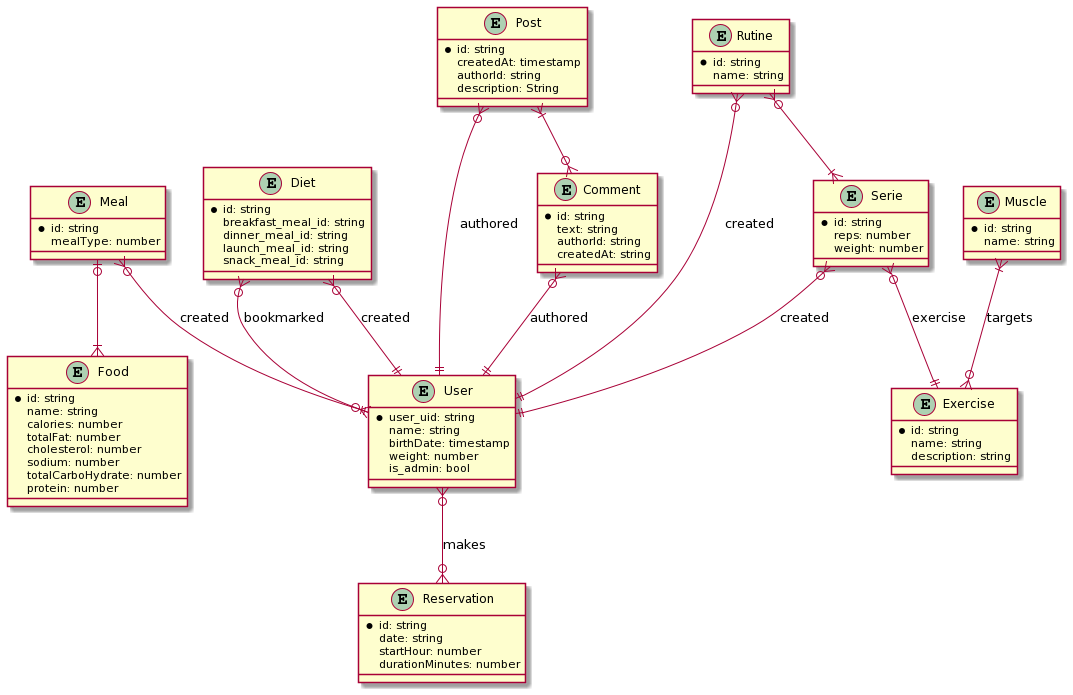
\includegraphics[width=0.6\textwidth]{diagramaer}
	\caption{Diagrama Entidad Relacion}
\end{figure}

\newpage

\section{Diseño}
TODO: Explicar la idea principal del diseño

\subsection{Colores}
TODO: explicar los colores utilizados


\subsection{Mockup}
\href{https://mockittapp.wondershare.com/app/3398ef738f7ac4f35fae5df4eb77004473612d19?simulator_type=device&sticky}{Link al mockup}

todo: poner foto

\newpage

\section{Estadísticas sobre el proyecto}

\subsection{Contribuciones}

\begin{figure}[h]
 	\centering
	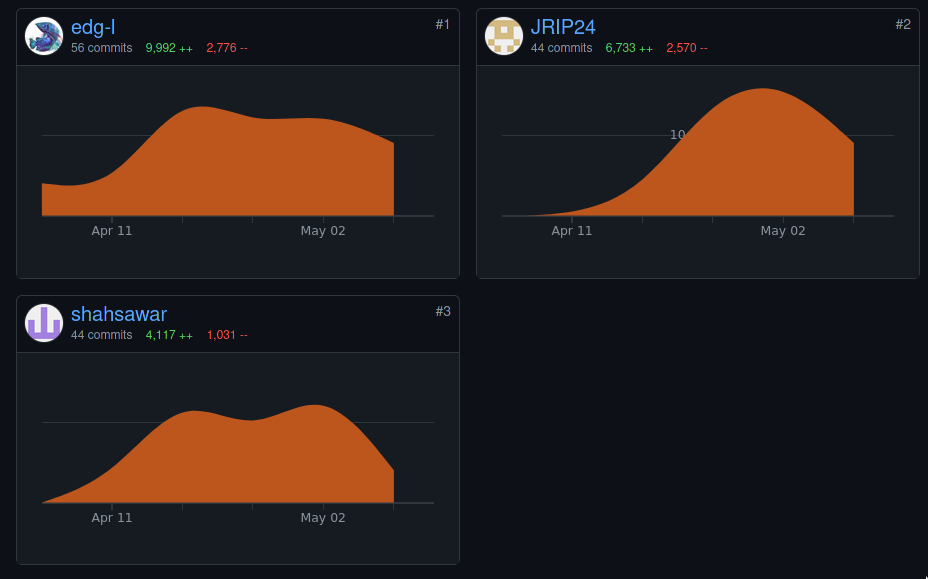
\includegraphics[width=\textwidth]{git-contributors}
	\caption{edg-l = Edgar, JRIP24 = Ronald, shasawar = Shah}
\end{figure}

\subsection{Lineas de código}

\begin{verbatim}
===============================================================================
 Language            Files        Lines         Code     Comments       Blanks
===============================================================================
 Batch                   1           84           61            0           23
 Java                   69         8648         5670         1453         1525
 JSON                    1           47           47            0            0
 Markdown                1            2            0            2            0
 Prolog                  1           21           18            0            3
 Shell                   1          172          130           23           19
 TeX                     1          200          136            0           64
 XML                    96         4280         3760          100          420
===============================================================================
 Total                 171        13454         9822         1578         2054
===============================================================================
\end{verbatim}

\newpage

\section{Conclusión}

\subsection{Posibles ampliaciones}

\subsubsection{Ampliar los datos de la comida}
Se podrían mostrar mas datos sobre la comida que se escanea, y a partir de estos datos llegar a conclusiones útiles para el usuario.

\end{document}